% !TeX root = er.tex

\chapter{Machine Learning}\label{ch.machine}

Consider a robot that recognizes and grasps yellow objects (Fig.~\ref{fig.sortballs}). It can use a color camera to identify yellow objects, but the objects will appear different in different environments, such as in sunlight, in a dark room, or in a showroom. Furthermore, it is hard to precisely define what ``yellow'' means: what is the boundary between yellow and lemon-yellow or between yellow and orange? Rather than write detailed instructions for the robot, we would prefer that the robot learn color recognition as it is performing the task, so that it  could adapt to the environment where the task takes place. Specifically, we want to design a \emph{classification algorithm} that can be \emph{trained} to perform the task without supplying all the details in advance.

\begin{figure}
\begin{center}
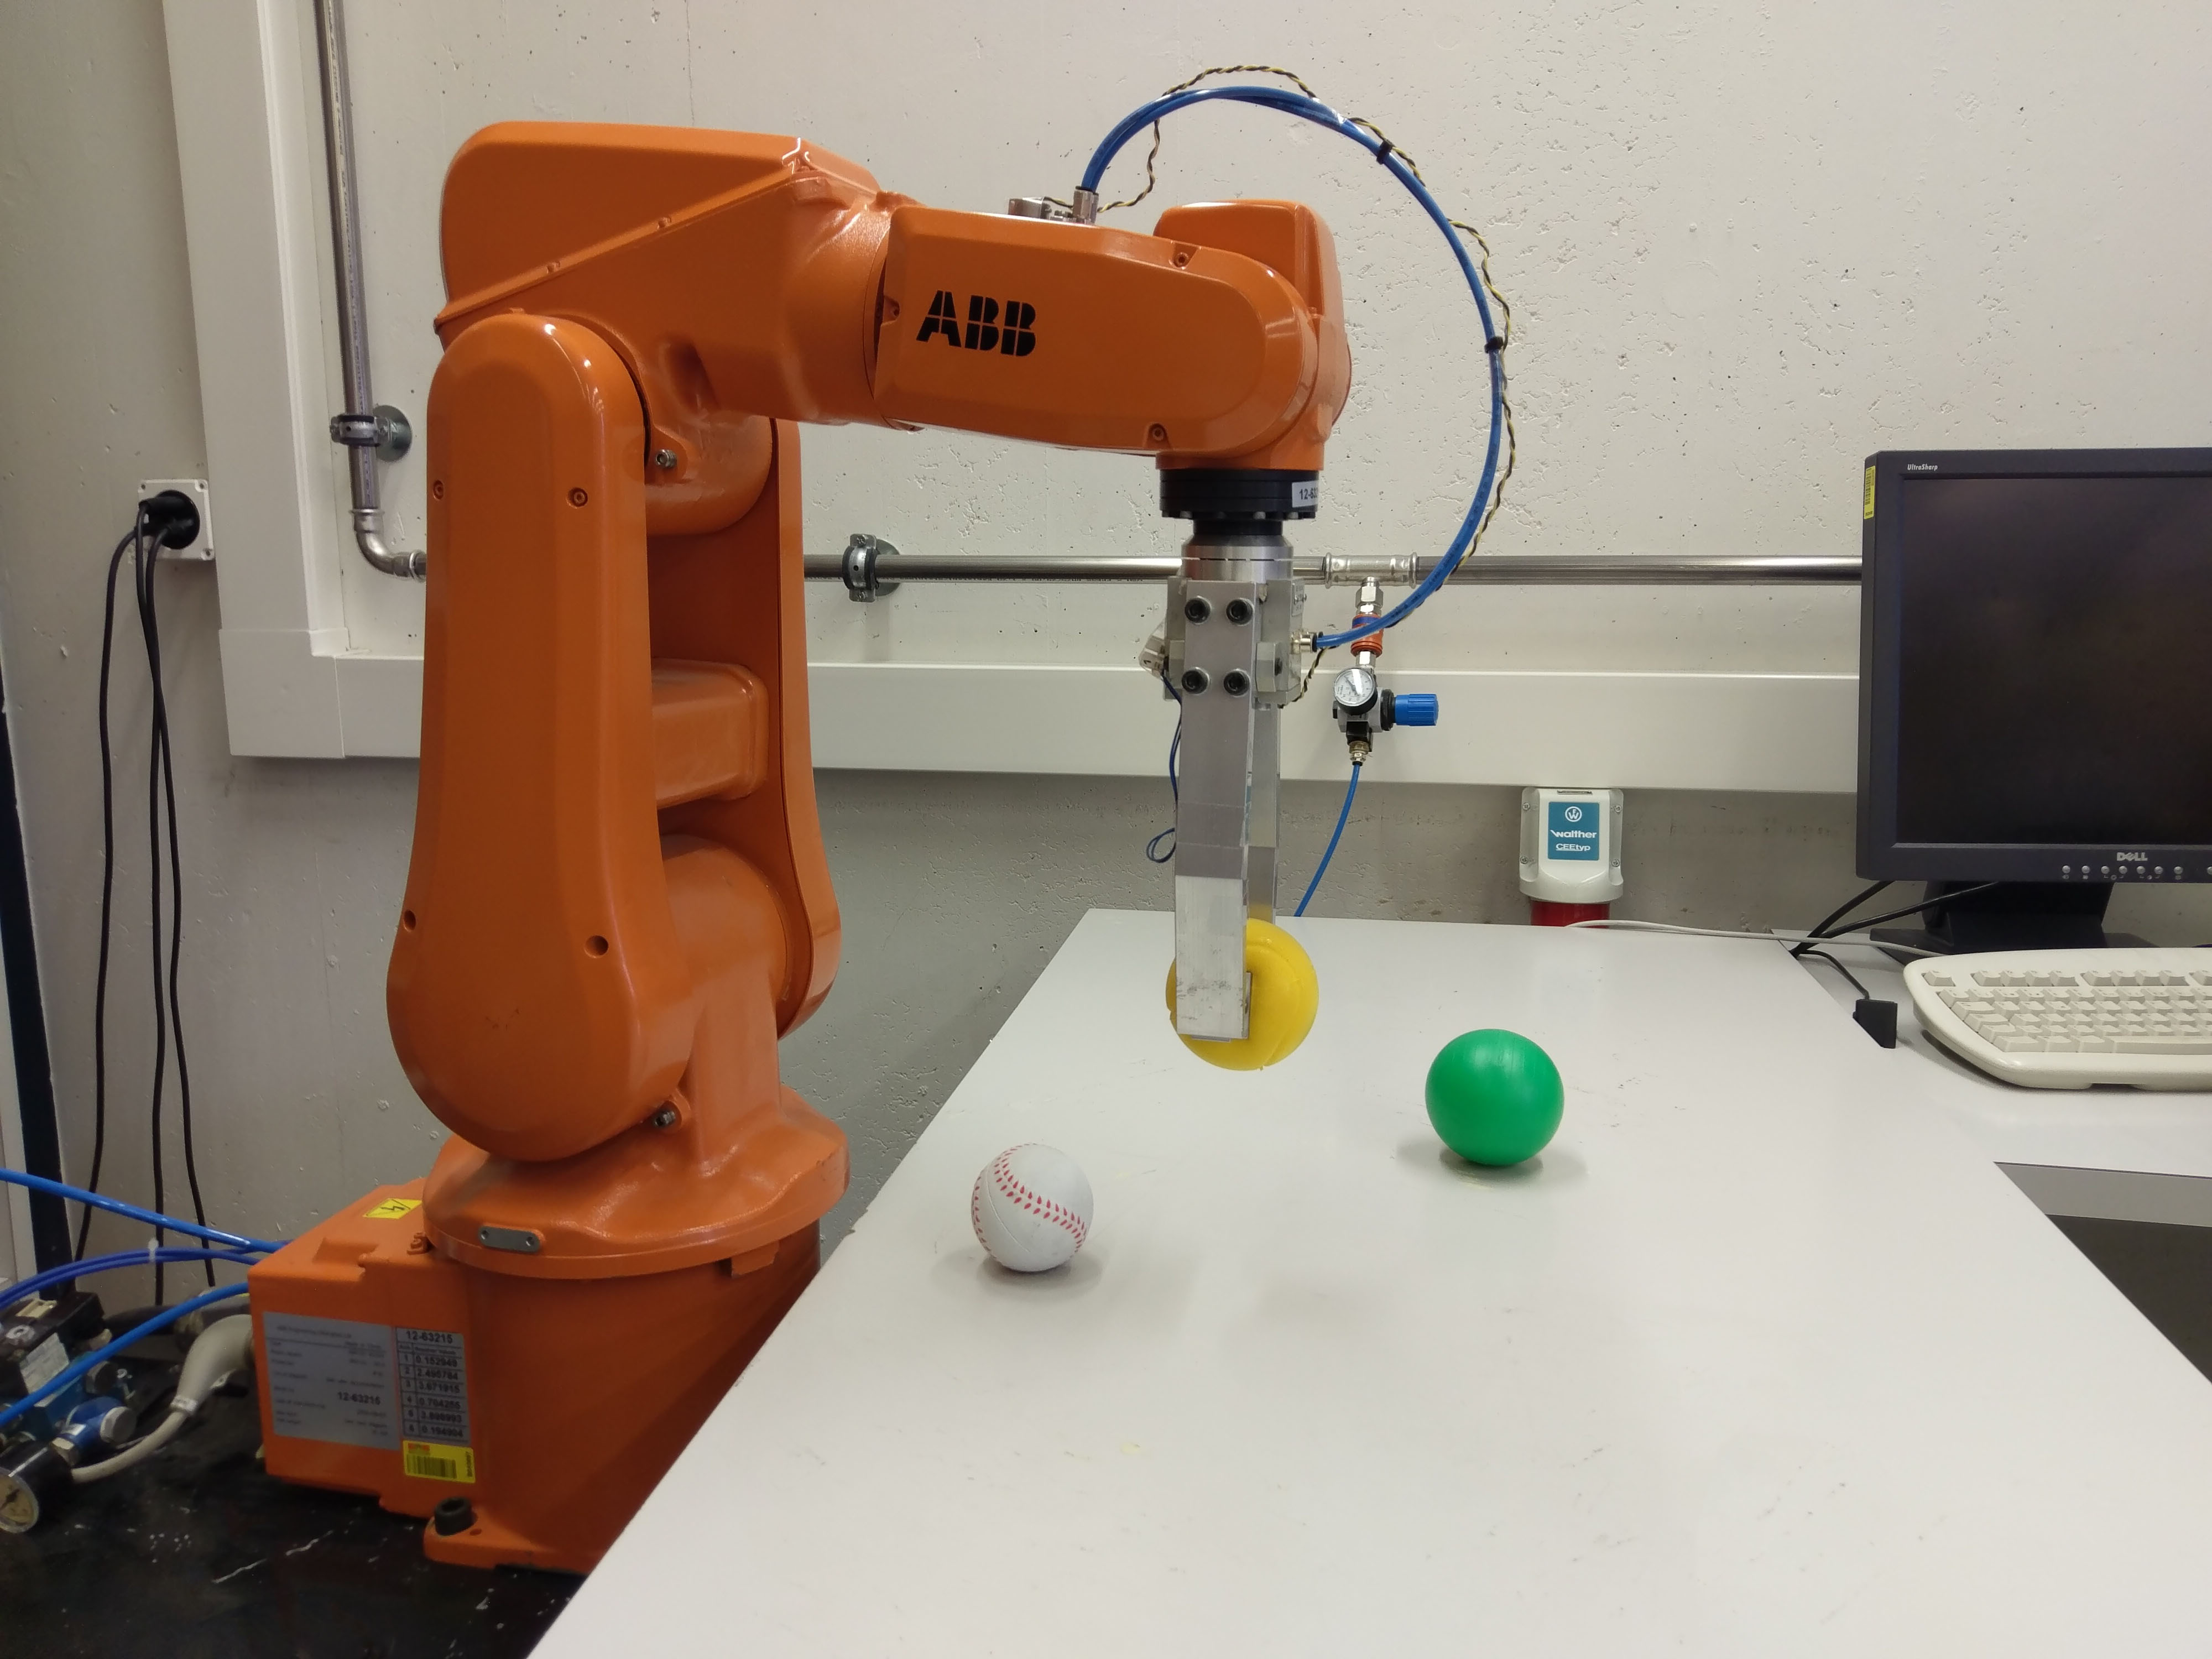
\includegraphics[width=0.8\textwidth]{sorting-robot.jpg}
\end{center}
\caption{Robotic arm sorting colored balls}\label{fig.sortballs}
\end{figure}

Classifications algorithms are a central topic in \emph{machine learning}, a field of computer science and statistics that develops computations to recognize patterns and to predict outcomes without explicit programming. These algorithms extract \emph{rules} from the raw data acquired by the system during a training period. The rules are subsequently used to classify a new object and then to take the appropriate action according to the class of the object. For the color-recognition task, we train the robot by presenting it with objects of different colors and telling the robot which objects are yellow and which are not. The machine learning algorithm generates a rule for color classification. When presented with new objects, it uses the rule to decide which objects are yellow and which are not.

The previous chapter presented artificial neural networks which perform a form of machine learning based upon \emph{reinforcement}. In this chapter, we discuss statistical techniques based upon \emph{supervised learning}: during the training period we tell the robot the precise answers, such as whether an object is yellow or not. Section~\ref{s.sorting-onesensor} introduces the statistical techniques by developing an algorithm for distinguishing between objects of two colors. We present a technique for machine learning called \emph{linear discriminant analysis (LDA)}. Sections~\ref{s.lda}--\ref{s.gen-lda} present LDA in the same context of distinguishing between two colors. LDA is based on the assumption that the data has specific statistical properties; if these do not hold, \emph{perceptrons} can be used for classification as described in Sect.~\ref{s.perceptrons}.

This chapter assumes that you are familiar with the concepts of \emph{mean}, \emph{variance} and \emph{covariance}. Tutorials on these concepts appear in Appendices~\ref{a.mean}--\ref{a.covariance}.

\section{Distinguishing between two colors}\label{s.sorting-onesensor}

We start with the problem of distinguishing yellow balls from non-yellow balls. To simplify the task, we modify the problem to one of distinguishing dark gray areas from light gray areas that are printed on paper taped to the floor (Fig.~\ref{fig.closegrays1}). The robot uses two ground sensors that sample the reflected light as the robot moves over the two areas.

\begin{figure}
\begin{center}
\begin{tikzpicture}[scale=.8]
\pic at (-2.2,1) { robot };
\draw[fill,gray] (-1,.6) rectangle +(6pt,8pt);
\draw[fill,gray] (-1,1.2) rectangle +(6pt,8pt);
\draw[fill,color=black!60]  (0,0) rectangle +(3.5,2);
\draw[fill,color=black!20] (4,0) rectangle +(3.5,2);
\end{tikzpicture}
\end{center}
\caption{Distinguishing two shades of gray}\label{fig.closegrays1}
\end{figure}

Figure~\ref{fig.closegrays2} shows a plot of the values returned by sampling the two sensors.\footnote{The data used in this chapter are real data taken from an experiment with the Thymio robot.} The robot takes about $70$ seconds to move from left to right, sampling the reflected light once per second. It is easy to see that the data shows significant variation, which is probably due to noise in the sensors and uneven printing. Even more problematic is the variability in the results returned by the two sensors. How can the robot learn to distinguish between the shades of gray given the variability in the samples and the sensors? We want to automatically create a rule to distinguish between the two shades of gray.

\begin{figure}
\begin{center}
\includegraphics[width=0.8\textwidth]{gray-fig.pdf}
\end{center}
\caption{Plots of reflected light vs. time for the left sensor (top) and the right sensor (bottom)}\label{fig.closegrays2}
\end{figure}

\subsection{A discriminant based on the means}

By examining the plots in Fig.~\ref{fig.closegrays2}, it is easy to see which samples are from the dark gray area and which are from the light gray area. For the left sensor, the values of the light gray area are in the range $500$--$550$, while the values of the dark gray area are in the range $410$--$460$. For the right sensor, the ranges are $460$--$480$ and $380$--$400$. For the left sensor, a threshold of $480$ would clearly distinguish between light and dark gray, while for the right sensor a threshold of $440$ would clearly distinguish between light and dark gray. But how can these optimal values be chosen automatically and how can we reconcile the thresholds of the two sensors?

Let us first focus on the left sensor. We are looking for a \textit{discriminant}, a value that distinguishes samples from the two colors. Consider the values $\mathit{max}_\sub{dark}$, the maximum value returned by sampling dark gray, and $\mathit{min}_{\sub{light}}$, the minimum value returned by sampling light gray. Under the reasonable assumption that $\mathit{max}_\sub{dark} < \mathit{min}_\sub{light}$, any value $x$ such that $\mathit{max}_\sub{dark} < x < \mathit{min}_\sub{light}$ can distinguish between the two shades of gray. The midpoint between the two values would seem to offer the most robust discriminant.

From Fig.~\ref{fig.closegrays2} we see that $\mathit{max}_\sub{dark}\approx 460$ occurs at about $10$ s and $\mathit{min}_{\sub{light}}\approx 500$ occurs at about $60$ s, so we choose their average $480$ as the discriminant. While this is correct for this particular data set, in general it is not a good idea to use the maximum and minimum values because they could be \emph{outliers}: extreme values resulting from unusual circumstances, such as a hole in the paper which would incorrectly return a very high value in the dark gray area.

A better solution is to use \emph{all} the data and the simplest function of all the data is the \emph{mean} of the values. Let $\mu_{\sub{dark}}$ denote the mean of the dark gray samples and $\mu_{\sub{light}}$ the mean of the light gray samples. A good discriminant $\Delta$ is the midpoint between the two means:
\begin{displaymath}
\Delta = \frac{\mu_{\sub{dark}} + \mu_{\sub{light}}}{2}\,.%\label{eq.discriminant}
\end{displaymath}
For the data in Fig.~\ref{fig.closegrays2} the means for the left sensor and the discriminant are:\footnote{In this chapter, values will be rounded to the nearest integer.}
\[
\mu_{\sub{dark}}^{\sub{left}} = 431,\;\;
\mu_{\sub{light}}^{\sub{left}} = 519,\;\;
\Delta^{\sub{left}} = \frac{431+519}{2} = 475\,.
\]
A similar computation gives the discriminant for the right sensor:
\[
\Delta^{\sub{right}} = 425\,.
\]

In order to obtain optimal recognition, we want an algorithm that is able to automatically decide which of the two discriminants is better. This is a preliminary stepping stone to the method described in Sect.~\ref{s.lda}, where a discriminant is computed by combining data from both sensors.

Intuitively, the greater the difference between the means of the light and dark areas:
\[
\left|\,\mu_{\sub{dark}}^{\sub{left}} - \mu_{\sub{light}}^{\sub{left}}\,\right|,\;\;\left|\,\mu_{\sub{dark}}^{\sub{right}} - \mu_{\sub{light}}^{\sub{right}}\,\right|\,,
\]
the easier it will be to place a discriminant between the two classes. The difference between the means of the left sensor ($88$) is a bit greater than the difference between the means of the right sensor ($84$). This leads us to choose the discriminant ($475$) computed from the means of the left sensor. However, from the plot in Fig.~\ref{fig.closegraysmus} it appears that this might not be the best choice because of the large variation in the samples of the left sensor.

\begin{figure}
\begin{center}
\includegraphics[width=0.8\textwidth]{gray-fig-mus.pdf}
\end{center}
\caption{Figure~\ref{fig.closegrays2} with means (short dashes), variances (brackets), discriminants (long dashes)}\label{fig.closegraysmus}
\end{figure}

\subsection{A discriminant based on the means and variances}

A better discriminant can be obtained if we consider not only the difference of the means but also the spread of the sample values around the mean. This is called the \emph{variance} of the samples. The variance $s^2$ of a set of values $\{x_1,x_2,\ldots,x_{n-1},x_n\}$ is:\footnote{Appendix~\ref{a.mean} explains why $n-1$ is used instead of $n$.}
\[
s^2 = \frac{1}{n-1} \sum_{i=1}^n (x_i-\mu)^2\,,
\]
where $\mu$ is the mean of the values in the set.

The variance computes the average of the distances of each sample from the mean of the samples. The distances are squared because a sample can be greater than or less than the mean, but we want a positive distance that shows how far the sample is from the mean.

The brackets in Fig.~\ref{fig.closegraysmus} show the four variances for the sets of samples of the light and dark areas for the left and right sensors.\footnote{Fig.~\ref{fig.closegraysmus} actually shows the square root of the variance called the standard deviation.} The difference between the left means is somewhat greater than the difference between the right means:
\[
\rule[-2ex]{0pt}{6ex}\left|\,\mu_{\sub{dark}}^{\sub{left}}-\mu_{\sub{light}}^{\sub{left}}\,\right| > \rule[-2ex]{0pt}{6ex}\left|\,\mu_{\sub{dark}}^{\sub{right}}-\mu_{\sub{light}}^{\sub{right}}\,\right|\,,
\]
but the variances of the right sensor are much smaller than the corresponding variances of the left sensor:
\[
\rule[-2ex]{0pt}{6ex}\left(s_{\sub{dark}}^{\sub{right}}\right)^2
\ll
\rule[-3ex]{0pt}{6ex}\left(s_{\sub{dark}}^{\sub{left}}\right)^2\,,\;\;\;
\rule[-2ex]{0pt}{6ex}\left(s_{\sub{light}}^{\sub{right}}\right)^2
\ll
\rule[-3ex]{0pt}{6ex}\left(s_{\sub{light}}^{\sub{left}}\right)^2\,.
\]
The use of the variances enables better classification of the two sets, since a sensor with less variance is more stable and this facilitates classification.

A good discriminant can be obtained by combining information from the means and the variances. The quality of a discriminant $J_k$, for $k=\mathit{left},\mathit{right}$, is given by:
\begin{equation}
J_k = \frac{\left(\mu_{\sub{dark}}^k - \mu_{\sub{light}}^k\right)^2}{\left(s_{\sub{dark}}^k\right)^2 + \left(s_{\sub{light}}^k\right)^2}\,.\label{eq.j}
\end{equation}
To maximize $J$, the numerator---the distance between the means---should be large, and the denominator---the variances of the samples---should be small.

Table~\ref{table.mu-s-j} displays the computations for the data set from Fig.~\ref{fig.closegraysmus}. The quality criterion $J$ for the right sensor is much larger than the one for the left sensor. It follows that the midpoint between the means of the right sensor:
\[
\Delta^{\sub{right}}=\frac{383+467}{2}=425
\]
is a better discriminant than the midpoint of the means of the left sensor that would be chosen by considering only the differences of the means $|\mu_{\sub{dark}}-\mu_{\sub{light}}|$, which is slightly larger for the left sensor than for the right sensor.

\begin{table}
\caption{The difference of the means and the quality criteria $J$}
\label{table.mu-s-j}
\begin{tabular}{p{2.5cm}p{3cm}p{3cm}p{3cm}p{3cm}}
\hline\noalign{\smallskip}
& \multicolumn{2}{r@{\hspace{1em}}}{left} & \multicolumn{2}{r@{\hspace{1em}}}{right} \\
\noalign{\smallskip}\hline\noalign{\smallskip}
& \multicolumn{1}{r}{dark} & \multicolumn{1}{r}{light} & \multicolumn{1}{@{\hspace{3em}}r}{dark} & \multicolumn{1}{r}{light}\\
\noalign{\smallskip}\hline\noalign{\smallskip}
$\mu$ & \multicolumn{1}{r}{$431$} & \multicolumn{1}{r}{$519$} & \multicolumn{1}{r}{$383$} & \multicolumn{1}{r}{$467$}\\
$s^2$ & \multicolumn{1}{r}{$121$} & \multicolumn{1}{r}{$225$} & \multicolumn{1}{r}{$16$} & \multicolumn{1}{r}{$49$}\\
$|\mu_{\sub{dark}}-\mu_{\sub{light}}|$ & \multicolumn{2}{r}{$88$} & \multicolumn{2}{r}{$84$}\\
$J$ & \multicolumn{2}{r}{$22$} & \multicolumn{2}{r}{$104$}\\
\noalign{\smallskip}\hline\noalign{\smallskip}
\end{tabular}
\end{table}

\subsection{Algorithm for learning to distinguish colors}

These computations are done by the robot itself, so the choice of the better discriminant and the better sensor is automatic. The details of the computation are given in Algorithms~\ref{alg.learning1}--\ref{alg.recognition1}.\footnote{Boldface variables represent vectors or matrices.}

There are two classes $C_1$, $C_2$ and two sensors. During the learning phase, the robot samples areas of the two gray levels independently and then computes the criterion of quality $J$. The sampling and computation are done for each sensor, either one after another or simultaneously. After the learning phase, the robot uses midpoint of the means with the best $J$ value for recognition of gray levels.

\begin{figure}
\begin{alg}{Distinguishing classes (learning phase)}{learning1}
&\idv{}float $\vec{X_1}, \vec{X_2}$&// Sets of samples\\
&\idv{}float $\mu_1,\mu_2$& // Means of $C_1,C_2$\\
&\idv{}float $s_1,s_2$& // Variances of $C_1,C_2$\\
&\idv{}float $\mu[2]$& // Means of $\mu_1,\mu_2$\\
&\idv{}float $J[2]$& // Criteria of quality\\
&\idv{}integer $k$& // Index of max($J[1],J[2]$)\\
\hline
\stl{}&for sensor i=1, 2&\\
\stl{}&\idc{}Collect a set of samples $\vec{X_1}$ from $C_1$&\\
\stl{}&\idc{}Collect a set  of samples $\vec{X_2}$ from $C_2$&\\
\stl{}&\idc{}Compute means $\mu_1$ of $\vec{X_1}$ and $\mu_2$ of $\vec{X_2}$&\\
\stl{}&\idc{}Compute variances $s_1$ of $\vec{X_1}$ and $s_2$ of $\vec{X_2}$&\\
\stl{}&\idc{}Compute the mean $\mu[i] = \displaystyle\frac{\mu_1 + \mu_2}{2}$&\\
\stl{}&\idc{}Compute the criterion $J[i]$ from Eq.~\ref{eq.j}&\\
\stl{}&$k$ \ass index of max($J[1],J[2]$)&\\
\stl{}&Output $\mu[k],k$&\\
\end{alg}
\end{figure}

\begin{figure}
\begin{alg}{Distinguishing classes (recognition phase)}{recognition1}
&\idv{}float $\mu$ \ass input $\mu[k]$ from the learning phase&\\
&\idv{}float x&\\
\hline
\stl{}&loop&\\
\stl{}&\idc{}$x$ \ass get new sample&\\
\stl{}&\idc{}if $x < \mu$&\\
\stl{}&\idc{}\idc{}assign $x$ to class $C_1$&\\
\stl{}&\idc{}else&\\
\stl{}&\idc{}\idc{}assign $x$ to class $C_2$&\\
\end{alg}
\end{figure}

\begin{framed}
\act{Robotic chameleon}{chameleon}
\begin{itemize}
\item Construct an environment as shown in Fig.~\ref{fig.closegrays1}. Print two pieces of paper with different uniform gray levels and tape them to the floor.
\item Write a program that causes the robot to move at a constant speed over the area of one color and sample the reflected light periodically. Repeat for the other color.
\item Plot the data, compute the means and the discriminant.
\item Implement a program that classifies the measurements of the sensor. When the robot classifies a measurement it displays which color is recognized like a chameleon (or gives other feedback if changing color cannot be done).
\item Apply the same method with a second sensor and compare the separability of the classes using the criterion $J$.
\item Repeat the exercise with two very close levels of gray. What do you observe?
\end{itemize}
\end{framed}

\section{Linear discriminant analysis}\label{s.lda}


In the previous section we classified samples of two levels of gray based on the measurements of one sensor out of two; the sensor was chosen automatically based on a quality criterion. This approach is simple but not optimal. Instead of choosing a discriminant based on one sensor, we can achieve better recognition by combining samples from both sensors. One method is called \emph{linear discriminant analysis (LDA)} and is based upon pioneering work in 1936 by the statistician Ronald A. Fisher.

\subsection{Motivation}

To understand the advantages of combining samples from two sensors, suppose that we need to classify objects of two colors: \emph{electric violet (ev)} and \emph{cadmium red (cr)}. Electric violet is composed largely of blue with a bit of red, while cadmium red is composed largely of red with a bit of blue. Two sensors are used: one measures the level of red and the other measures the level of blue. For a set of samples, we can compute their means $\mu_j^k$ and variances $(s_j^k)^2$, for $j=\mathit{ev}, \mathit{cr}$, $k=\mathit{blue}, \mathit{red}$.

The left plot in Fig.~\ref{fig.LDAprincipe} shows samples of the electric violet objects contained within a dashed ellipse at the upper left and samples of the cadmium red objects contained within a dashed ellipse at the lower right. The centers of the ellipses are the means because the samples are symmetrically distributed with respect to the ellipses. The $y$-coordinate of $\mu_{ev}$ is the mean of the samples of the electric violet objects by the blue sensor and its $x$-coordinate is the mean of the samples of these objects by the red sensor. The means of the sensors when sampling the cadmium red objects are similarly displayed. It is easy to see  that the electric violet objects have more blue (they are higher up the $y$-axis), while the cadmium red objects have more red (they are further out on the $x$-axis).

\begin{figure}
\begin{center}
\includegraphics[width=\textwidth]{LDA-principe-colors2.pdf}
\end{center}
\caption{An optimal linear discriminant for distinguishing two colors}\label{fig.LDAprincipe}
\end{figure}

From the diagram we see that there is a larger difference between the means for the blue sensor than between the means for the red sensor. At first glance, it appears that using the blue sensor only would give a better discriminant. However, this is not true: the dashed lines show that the red-only discriminant completely distinguishes between electric violet and cadmium red, while the blue-only discriminant falsely classifies some electric violet samples as cadmium red (some samples are below the line) and falsely classifies some cadmium red samples as electric violet (some samples are above the line).

The reason for this unintuitive result is that the blue sensor returns values that are widely spread out (have a large variance), while the red sensor returns values that are narrowly spread out (have a small variance), and we saw in Sect.~\ref{s.sorting-onesensor} that classification is better if the variance is small. The right plot in Fig.~\ref{fig.LDAprincipe} shows that by constructing a discriminant from both sensors it is possible to better separate the electric violet objects from the cadmium red objects. The discriminant is still linear (a straight line) but its slope is no longer parallel to one of the axes. This line is computed using the variances as well as the means. The method is called linear discriminant analysis because the discriminant is linear.


\subsection{The linear discriminant}
Figure~\ref{fig.LDAprincipe} is an $x$-$y$ plot of data sampled from two sensors. Each value is plotted at the point whose $x$-coordinate is the value returned by the red sensor and whose $y$-coordinate is the value returned by the blue sensor. Similarly, Fig.~\ref{fig.gray-x-y} is an $x$-$y$ plot of the data from Figs.~\ref{fig.closegrays2}--\ref{fig.closegraysmus} that were collected as the robot moved over two gray areas.  In those graphs, the sensor values were plotted as function of time, but time has no role in classification except to link samples that were measured at the same time by the two sensors.

\begin{figure}
\begin{center}
\includegraphics[width=\textwidth]{gray-level-base.pdf}
\end{center}
\caption{$x$-$y$ plot of gray levels with single-sensor discriminants and an optimal discriminant}\label{fig.gray-x-y}.
\end{figure}

In Fig.~\ref{fig.gray-x-y}, classification based only on the left sensor corresponds to the vertical dashed line, while classification based only on the right sensor corresponds to the horizontal dashed line. Both the horizontal and vertical separation lines are not optimal. Suppose that classification based on the left sensor (the vertical line) is used and consider a sample for which the left sensor returns $470$ and the right sensor returns $460$. The sample will be classified as dark gray even though the classification as light gray is better. Intuitively, it is clear that the solid diagonal line in the graph is a far more accurate discriminant than either of the two discriminants based on a single sensor.

How can such a linear discriminant be defined mathematically so that it can be discovered automatically?\footnote{The following presentation is abstract and will be easier to understand if read together with the numerical example in Sect.~\ref{s.num-lda}.} The general equation for a line in the plane is $y=mx+a$, where $m$ is the slope and $a$ is the intersect of the line and the $y$-axis when $x=0$. Another equation for a line is:
\begin{equation}
w_1x_1 + w_2x_2 = c\,,\label{eq.diseq}
\end{equation}
where $x_1$ is the horizontal axis for the left sensor values, $x_2$ is the vertical axis for the right sensor values. $c$ is a constant and $w_1,w_2$ are coefficients of the variables.

It is convenient to represent the coefficients as a column vector:
\[
\vec{w} = \left[ \begin{array}{c} w_1\\w_2 \end{array} \right]\,.
\]
In this representation the vector $\vec{w}$ is normal to the discriminant line and therefore defines its slope, while the constant $c$ enables the discriminant to be any line of that slope, that is, any one of the infinite number of parallel lines with a given slope. Once the slope of $\vec{w}$ is determined, $c$ is obtained by entering a given point ($x_1$,$x_2$) into Eq.~\ref{eq.diseq}.

Linear discriminant analysis automatically defines the vector $\vec{w}$ and constant $c$ that generates an optimal discriminant line between the data sets of the two classes. The first step is to choose a point on the discriminant line. Through that point there are an infinite number of lines and we have to choose the line whose slope gives the optimal discriminant. Finally, the value $c$ can be computed from the slope and the chosen point. The following subsections describe each of these steps in detail.

\subsection{Choosing a point for the linear discriminant}

How can we choose a point? LDA is based upon the \emph{assumption} that the values of both classes have the same distribution. Informally, when looking at an $x$-$y$ plot, both sets of points should have similar size and shape. Although the distributions will almost certainly not be exactly the same (say a Gaussian distribution) because they result from measurements in the real world, since both sensors are subject to the same types of variability (sensor noise, uneven floor surface) it is likely that they will be similar.

If the two distributions are similar, the means of the samples of each sensor will be more-or-less in the same place with respect to the distributions. The average of the means for each sensor will be equidistant from corresponding points in the data sets. The discriminant is chosen to be some line that passes through the point $M$ (Fig.~\ref{fig.gray-x-y}) whose coordinates are:
\[
\left(\,
\frac{\mu_{\sub{light}}^{\sub{left }}+\mu_{\sub{dark}}^{\sub{left }}}{2},\:\frac{\mu_{\sub{light}}^{\sub{right}}+\mu_{\sub{dark}}^{\sub{right}}}{2}
\,\right)\,.
\]

\subsection{Choosing a slope for the linear discriminant}

Once we have chosen the point $M$ on the discriminant line, the next step is to choose the slope of the line. From Fig.~\ref{fig.gray-x-y}, we see that there are infinitely many lines through the point $M$ that would distinguish between the two sets of samples. Which is the best line based on the statistical properties of our data?

In Sect.~\ref{s.sorting-onesensor} we looked for a way to decide between two discriminants, where each discriminant was a line parallel to the $y$-axis at the midpoint between the means of the values returned by a sensor (Fig.~\ref{fig.closegraysmus}). The decision was based on the quality criterion $J_k$ (Eq.~\ref{eq.j}, repeated here for convenience):
\begin{equation}
J_k = \frac{\left(\mu_{\sub{dark}}^k - \mu_{\sub{light}}^k\right)^2}{\left(s_{\sub{dark}}^k\right)^2 + \left(s_{\sub{light}}^k\right)^2}\,,\label{eq.j-repeat}
\end{equation}
where $k=\textit{left},\textit{right}$. The discriminant with the larger value of $J_k$ was chosen. To maximize $J_k$, the numerator---the distance between the means---should be large, and the denominator---the variances of the samples---should be small.

Now, we no longer want to compute a quality criterion based on the values returned by each sensor separately, but instead to compute a criterion from all the values returned by both sensors. Figure~\ref{fig.lda-proj} shows an $x$-$y$ plot of the values of two sensors, where the values of the two classes are represented by red squares and blue circles. Clearly, there is significant overlap along the $x$ or $y$ axes separately and it is impossible to find lines parallel to the axes that can distinguish between the groups. However, if we project the groups of measurements onto the line defined by a vector:
\[
\vec{w} = \left[\begin{array}{c}w_1\\w_2\end{array}\right]\,,
\]
the two groups can be distinguished by the separator line defined by Eq.~\ref{eq.diseq}:
\[
w_1x_1 + w_2x_2 = c\,,
\]
where $c$ is defined by a point on the project line situated between the red and blue points. In analogy with Eq.~\ref{eq.j-repeat}, we need to define a quality criterion $J(\vec{w})$, such that larger values of $J(\vec{w})$ give better discriminant lines. Then, we need to find the value of $\vec{w}$ that maximizes $J(\vec{w})$ by differentiating this function, setting the derivative to zero and solving for $\vec{w}$.

\begin{figure}
\begin{center}
\includegraphics[width=0.9\textwidth]{LDA-principe-proj3.pdf}
\end{center}
\caption{Projection of the samples of two classes onto a line defined by $\vec{w}$}\label{fig.lda-proj}
\end{figure}

The definition of $J(\vec{w})$ is based on the means and variances of the two classes but is too complex for this book. We give without proof that the value of $\vec{w}$ that maximizes $J(\vec{w})$ is:
\begin{equation}
\vec{w} = \vec{S}^{-1}\,(\vec{\mu_{\sub{light}}}-\vec{\mu_{\sub{dark}}})\,,\label{eq.wLDA}
\end{equation}
where:
\[
\renewcommand{\arraystretch}{1.8}
\vec{\mu_{\sub{light}}}=\left[
\begin{array}{c}\mu_{\sub{light}}^{\sub{left}}\\
\mu_{\sub{light}}^{\sub{right}}\end{array}
\right]\,,\;\;\;
\vec{\mu_{\sub{dark}}}=\left[
\begin{array}{c}\mu_{\sub{dark}}^{\sub{left}}\\
\mu_{\sub{dark}}^{\sub{right}}\end{array}\right]
\]
are the mean vectors of the two classes and $\vec{S}^{-1}$ is the inverse of the average of the covariance matrices of the two classes:\footnote{See Appendix~\ref{a.covariance} for the definition of covariance and Sect.~\ref{s.num-lda} for a numerical example that will clarify the computations.}
\[
\renewcommand{\arraystretch}{2.5}
\vec{S} = \frac{1}{2}\left(
\left[\begin{array}{l@{\hspace{.4em}}l}
s^2\left(\vec{x^{\sub{left}}_\sub{light}}\right) &
\textit{cov}\left(\vec{x^{\sub{left}}_\sub{light}},\vec{x^{\sub{right}}_\sub{light}}\right)\\
\textit{cov}\left(\vec{x^{\sub{right}}_\sub{light}},\vec{x^{\sub{left}}_\sub{light}}\right)&
s^2\left(\vec{x^{\sub{right}}_\sub{light}}\right)
\end{array}\right]
\!+\!
\left[\begin{array}{l@{\hspace{.5em}}l}
s^2\left(\vec{x^{\sub{left}}_\sub{dark}}\right)&
\textit{cov}\left(\vec{x^{\sub{left}}_\sub{dark}},\vec{x^{\sub{right}}_\sub{dark}}\right)\\
\textit{cov}\left(\vec{x^{\sub{right}}_\sub{dark}},\vec{x^{\sub{left}}_\sub{dark}}\right)&
s^2\left(\vec{x^{\sub{right}}_\sub{dark}}\right)
\end{array}\right]\right).
\]
Compared with the single-sensor $J_k$, the means are two-dimensional vectors because we have one mean for each of the sensors. The sum of variances becomes the covariance matrix, which takes into account both the individual variances of the two sensors and the covariances that express how the two sensors are related.

When the values of $M$ and $\vec{w}$ have been computed, all that remains is to compute the constant $c$ to fully define the discriminant line. This completes the learning phase of the LDA algorithm. In the recognition phase, the robot uses the line defined by $\vec{w}$ and $c$ for classifying new samples.

The computation is formalized in Algorithms~\ref{alg.learning2}--\ref{alg.recognition2}, where we want to distinguish between two classes $C_1, C_2$ using two sensors. Compare this algorithm with Algorithm~\ref{alg.learning1}: the two sets of samples $\vec{X_1},\vec{X_2}$ and the means $\vec{\mu_1},\vec{\mu_2}$ and variances $\vec{s_1},\vec{s_2}$ are vectors with two elements, one element for each of the sensors.

\begin{figure}
\begin{alg}{Linear discriminant analysis (learning phase)}{learning2}
&\idv{}float array[n$_1$,2] $\vec{X_1}$&// Sets of samples of first area\\
&\idv{}float array[n$_2$,2] $\vec{X_2}$&// Sets of samples of second area\\
&\idv{}float array[2] $\vec{\mu_1},\vec{\mu_2}$& // Means of $C_1,C_2$\\
&\idv{}float array[2] $\vec{\mu}$& // Mean of the means\\
&\idv{}float array[2] $\vec{s_1},\vec{s_2}$& // Variances of $C_1,C_2$\\
&\idv{}float $cov_1,cov_2$& // Covariances of $C_1,C_2$\\
&\idv{}float array[2] $\vec{S_\sub{inv}}$&// Inverse of average\\
&\idv{}float $c$& // Constant of the line\\
\hline
\stl{}&Collect a set of $n_1$ samples $\vec{X_1}$ from $C_1$&\\
\stl{}&Collect a set  of $n_2$ samples $\vec{X_2}$ from $C_2$&\\
\stl{}&Compute means $\vec{\mu_1}$ of $\vec{X_1}$ and $\vec{\mu_2}$ of $\vec{X_2}$&\\
\stl{}&$\vec{\mu}$ \ass{} $(\vec{\mu_1}+\vec{\mu_2})/2$&\\
\stl{}&Compute variances $\vec{s_1}$ of $\vec{X_1}$ and $\vec{s_2}$ of $\vec{X_2}$&\\
\stl{}&Compute covariances $cov_1,cov_2$ of $\vec{X_1}$ and $\vec{X_2}$&\\
\stl{}&Compute $\vec{S_\sub{inv}}$ of covariance matrix&\\
\stl{}&Compute $\vec{w}$ from Eq.~\ref{eq.wLDA}&\\
\stl{}&Compute point $M$ from $\vec{\mu}$&\\
\stl{}&Compute $c$ from $M$ and $\vec{w}$&\\
\stl{}&Ouptut $\vec{w}$ and $c$&\\
\end{alg}
\end{figure}

\begin{figure}
\begin{alg}{Linear discriminant analysis (recognition phase)}{recognition2}
&\idv{}float $\vec{w}$ \ass input from the learning phase&\\
&\idv{}float $c$ \ass input from the learning phase&\\
&\idv{}float $\vec{x}$&\\
\hline
\stl{}&loop&\\
\stl{}&\idc{}$\vec{x}$ \ass new sample&\\
\stl{}&\idc{}if $\vec{x}\cdot \vec{w} < c$&\\
\stl{}&\idc{}\idc{}assign $\vec{x}$ to class $C_1$&\\
\stl{}&\idc{}else&\\
\stl{}&\idc{}\idc{}assign $\vec{x}$ to class $C_2$&\\
\end{alg}
\end{figure}

\subsection{Computation of a linear discriminant: numerical example}\label{s.num-lda}


Figure~\ref{fig.gray-close} is a plot of the samples from two ground sensors measured as a robot moves over two very similar gray areas, one that is $83.6\%$ black and the other $85\%$ black. The levels are so close that the human eye cannot distinguish between them. Can the linear discriminant computed by Algorithm~\ref{alg.learning2} do better?

\begin{figure}
\begin{center}
\includegraphics[width=\textwidth]{close-gray.pdf}
\end{center}
\caption{Similar gray areas (black dots from the darker area, red x'es from the lighter area)}\label{fig.gray-close}
\end{figure}

Class $C_1$ is the light gray area and class $C_2$ is the dark gray area. The elements of the sets of vectors $\vec{X_1}[n_1],\vec{X_2}[n_2]$ are vectors:
\[
\vec{x}=\left[ \begin{array}{c} x^{\sub{left}} \\ x^{\sub{right}} \end{array} \right]
\]
of samples measured by the left and right sensors, where $n_1=192$ and $n_2=205$.

First we compute the means of the data of Fig.~\ref{fig.gray-close}:
\begin{displaymath}
\begin{array}{ccccc}
\vec{\mu_1} &=& {\displaystyle\frac{1}{192}} \left( \left[ \begin{array}{c} 389\\324 \end{array}\right] + \left[ \begin{array}{c} 390\\323 \end{array}\right] + ... + \left[ \begin{array}{c} 389\\373 \end{array}\right] \right)&\approx&\left[ \begin{array}{c} 400\\339 \end{array}\right]\\
\\
\vec{\mu_2} &=& {\displaystyle\frac{1}{205}} \left( \left[ \begin{array}{c} 358\\297 \end{array}\right] + \left[ \begin{array}{c} 358\\296 \end{array}\right] + ... + \left[ \begin{array}{c} 352\\327 \end{array}\right] \right)&\approx&\left[ \begin{array}{c} 357\\312 \end{array}\right]\,.
\end{array}
\end{displaymath}
More samples were taken from the second area ($205$) than from the first area ($192$), but that is not important for computing the means. As expected, the means $\vec{\mu_1}$ of the samples from the light gray area are slightly higher (more reflected light) than the means $\vec{\mu_2}$ of the samples from the dark gray areas. However, the left sensor consistently measures higher values than the right sensor. Figure~\ref{fig.gray-close-mu-lin} shows the data from Fig.~\ref{fig.gray-close} with thin dashed lines indicating the means. There are two lines for each area: the horizontal line for the right sensor and the vertical line for the left sensor.

\begin{figure}
\begin{center}
\includegraphics[width=\textwidth]{close-gray-mu-lin.pdf}
\end{center}
\caption{Means for each class (thin dashed lines), LDA discriminant line (solid line), discriminant line that fully distinguishes the classes (thick dashed line)}\label{fig.gray-close-mu-lin}
\end{figure}

The covariance matrix is composed from the variances of the two individual sensors and their covariance. For $i=1,2$:
\[
\vec{S}_i = \left[
\renewcommand{\arraystretch}{2}
\begin{array}{l@{\hspace{1em}}l}
s^2\left(X_i^{\sub{left}}\right) &
\textit{cov}\left(X_i^{\sub{left}}, X_i^{\sub{right}}\right)\\
\textit{cov}\left(X_i^{\sub{right}},X_i^{\sub{left}}\right)&
s^2\left(X_i^{\sub{right}}\right)
\end{array}
\right]\,.
\]
For the data from Fig.~\ref{fig.gray-close}, the variances of the samples of the light gray area are:
\begin{eqnarray*}
s^2(X_1^{\sub{left}}) &=& \frac{1}{191} \left((389 - 400)^2 + (390 - 400)^2 + \cdots + (389 - 400)^2 \right) \approx 187 \\
s^2(X_1^{\sub{right}}) &=& \frac{1}{191} \left((324 - 339)^2 + (323 - 339)^2 + ... + (373 - 339)^2 \right) \approx 286\,.
\end{eqnarray*}

Eq.~\ref{eq.cov} from Appendix~\ref{a.covariance} is used to compute the covariance. Since covariance is symmetric, the value need be computed only once.
\begin{eqnarray*}
\textit{cov}(X_1^{\sub{left}}, X_1^{\sub{right}}) &=& \frac{1}{191} \left((389 - 400)(324 - 339) + ... + (389 - 400)(373 - 339) \right)\\
&\approx& -118\,.
\end{eqnarray*}
Putting the results together and performing a similar computation for $X_2$ gives the covariance matrices:
\[
\vec{S}_1 = \left[ \begin{array}{c} 187\\-118\end{array} \begin{array}{c} -118\\286 \end{array}\right]
\hspace{10mm}
\vec{S}_2 = \left[ \begin{array}{c} 161\\44\end{array} \begin{array}{c} 44\\147 \end{array}\right]\,.
\]

The next step is to compute the mean of the covariance matrices:
\[
\mu_{\vec{S}} = 
\frac{1}{2}\left(\left[ \begin{array}{c} 187\\-118\end{array} \begin{array}{c} -118\\286 \end{array}\right]+
\left[ \begin{array}{c} 161\\44\end{array} \begin{array}{c} 44\\147 \end{array}\right]\right) = 
\left[ \begin{array}{c} 174\\-37\end{array} \begin{array}{c} -38\\216 \end{array}\right]\,,
\]
and to find its inverse:\footnote{See Appendix~\ref{a.matrices}.}
\[
\vec{S}^{-1} = \left[ \begin{array}{c} 0.006\\0.001\end{array} \begin{array}{c} 0.001\\0.005 \end{array}\right]\,.
\]
We can now use Eq.~\ref{eq.wLDA} to compute $\vec{w}$:
\[
\vec{w} = \left[ \begin{array}{c} 0.006\\0.001\end{array} \begin{array}{c} 0.001\\0.005 \end{array}\right] \cdot \left( \left[ \begin{array}{c} 400\\339 \end{array}\right] - \left[ \begin{array}{c} 357\\313 \end{array} \right] \right) = \left[ \begin{array}{c} 0.28\\0.17 \end{array} \right]\,.
\]
The vector $\vec{w}$ gives the direction of the projection line which is perpendicular to discriminant line. We now use Eq.~\ref{eq.diseq}, repeated here:
\[
w_1x_1 + w_2x_2 = c
\]
to compute the constant $c$, assuming we know the coordinate $(x_1,x_2)$ of some point. But we specified that the midpoint between the means must be on the discriminant line. Its coordinates are:
\[
\vec{\mu} = \frac{1}{2}(\vec{\mu_1} + \vec{\mu_2}) = \frac{1}{2}\left( \left[ \begin{array}{c} 400\\339 \end{array}\right] + \left[ \begin{array}{c} 357\\313 \end{array}\right] \right) \approx \left[ \begin{array}{c} 379\\326 \end{array}\right]\,.
\]
Therefore:
\[
c = 0.28 \cdot 379 + 0.17\cdot 326 \approx 162\,,
\]
and the equation of the discriminant line is:
\[
0.28 x_1 + 0.17 x_2 = 162\,.
\]
The discriminant line is shown as a solid line in Fig.~\ref{fig.gray-close-mu-lin}. Given a new sample $(a,b)$, compare the value of $0.28a + 0.17b$ to $162$: If it is larger, the sample is classified as belonging to class $C_1$ and if it is is smaller, the sample is classified as belong to class $C_2$. 

\subsection{Comparing the quality of the discriminants}

If we compare the linear discriminant found above with the two simple discriminants based upon the means of a single sensor, we see a clear improvement. Because of the overlap between the classes in a single direction, the simple discriminant for the right sensor correctly classifies only $84.1\%$ of the samples, while the simple discriminant for the left sensor is somewhat better, classifying $93.7\%$ of samples correctly. The linear discriminant found using LDA is better, correctly classifying $97.5\%$ of the samples.

It might be surprising that there are discriminant lines that can correctly classify \emph{all} of the samples! One such discriminant is shown by the thick dashed line in Fig.~\ref{fig.gray-close-mu-lin}. Why didn't LDA find this discriminant? LDA assumes both classes have a similar distribution (spread of values) around the mean and the LDA discriminant is optimal under this assumption. For our data, some points in the second class are far from the mean and thus the distributions of the two classes are slightly different. It is hard to say if these samples are outliers, perhaps caused by problem when printing the gray areas on paper. In that case, it is certainly possible that subsequent sampling of the two areas would result in distributions that are similar to each other, leading to the correct classification by the LDA discriminant.

\subsection{Activities for LDA}

Activities for LDA are collected in this section.

\begin{framed}
\act{Robotic chameleon with LDA}{LDAchameleon}
\begin{itemize}
\item Construct an environment as shown in Fig.~\ref{fig.closegrays1} but with two gray levels very similar to each other.
\item Write a program that causes the robot to move at a constant speed over the area of one color and sample the reflected light periodically. Repeat for the other color.
\item Plot the data.
\item Compute the averages, the covariance matrices and the discriminant. 
\item Implement a program that classifies measurements of the sensor. When the robot classifies a measurement it displays which color is recognized (or gives other feedback if changing color cannot be done).
\end{itemize}
\end{framed}

\begin{framed}
\act{Obstacle avoidance with two sensors}{LDAobstacle}
\begin{itemize}
\item Figure~\ref{fig.train-data-avoid} shows a robot approaching a wall. The upper part of the diagram shows various situations where the robot detects the wall with its right sensors; therefore, it should turn left to move around the wall. Similarly, in the lower part of the diagram the robot should turn right.
\item Write a program that stores the sensor values from both the right and left sensors when a button is pressed. The program also stores the identity of which button was pressed; this represents the class we are looking for when doing obstacle avoidance.
\item Train the robot: Place the robot next to a wall and run the program. Touch the left button if the robot should turn left or the right button if the robot should turn right. Repeat many times.
\item Plot the samples from the two sensors on an $x$-$y$ graph and group them by class: turn right or left to avoid of the wall. You should obtain a graph similar to the one in Fig.~\ref{fig.machlearnavoid}.
\item Draw a discriminant line separating the two classes.
\item How successful is your discriminant line? What percentage of the samples can it successfully classify?
\item Compute the optimal discriminant using LDA. How successful is it? Do the assumptions of LDA hold?
\end{itemize}
\end{framed}

\begin{figure}
\begin{center}
\begin{tikzpicture}[align=left]
\foreach \angle/\x in { 100/0cm, 120/2cm, 140/4cm, 110/6cm, 100/8cm } {
  \draw[fill] (\x,0) rectangle +(16mm,1mm);
  \pic[rotate=\angle,scale=0.4] at (\x+8mm, -8mm) { robot };
}
\node at (-1,-.5) {\textsf{Turn}\\\textsf{left}};
\foreach \angle/\x in { 70/0cm, 85/2cm, 65/4cm, 85/6cm, 75/8cm } {
  \draw[fill] (\x,-2.5) rectangle +(16mm,1mm);
  \pic[rotate=\angle,scale=0.4] at (\x+8mm, -33mm) { robot };
}
\node at (-1,-3) {\textsf{Turn}\\\textsf{right}};
\end{tikzpicture}
\end{center}
\caption{Training for obstacle avoidance}\label{fig.train-data-avoid}
\end{figure}

\begin{figure}
\begin{center}
\includegraphics[width=0.9\textwidth]{avoid-graph-classes.pdf}
\end{center}
\caption{Obstacle avoidance data from the class ``go left'' (red x'es) and the class ``go right'' (black triangles)}\label{fig.machlearnavoid}
\end{figure}

\begin{framed}
\act{Following an object}{follow}
\begin{itemize}
\item Write a program that causes the robot to follow an object. The robot moves forward if it detects the object in front; it moves backwards if it is  too close to the object. The robot turns right if the object is to its right and the robot turns left if the object is to its left.
\item Use two sensors so we can visualize the data on an $x$-$y$ plot.
\item Acquire and plot the data as in Activity~\ref{act.LDAobstacle}. The plot should be similar to the one shown in Fig.~\ref{fig.machlearnfollow}.
\item Explain the classifications in Fig.~\ref{fig.machlearnfollow}. What is the problem with classifying a sample as going forwards or going backwards? Why do the samples for going forwards and backwards have different values for the left and right sensors?
\item Suggest an algorithm for classifying the four situations. Could you use a combination of linear separators?
\end{itemize}
\end{framed}

\begin{figure}
\begin{center}
\includegraphics[width=\textwidth]{graph-follow-classes.pdf}
\end{center}
\caption{Data acquired in a learning phase for following an object}\label{fig.machlearnfollow}
\end{figure}

\section{Generalization of the linear discriminant}\label{s.gen-lda}

In this section we point out some ways in which LDA can be extended and improved.

First, we can have more sensors. The mathematics becomes more complex because with $n$ sensors, the vectors will have $n$ elements and the covariance matrix will have $n\times n$ elements, requiring more computing power and more memory. Instead of a discriminant line, the discriminant will be an $n-1$ dimension hyperplane. Classification with multiple sensors is used with electroencephalography (EEG) signals from the brain in order to control a robot by thought alone.

Activity~\ref{act.follow} demonstrated another generalization: classification into more than two classes. Discriminants are used to classify between each pair of classes. Suppose you have three classes $C_1$, $C_2$, and $C_3$, and discriminants $\Delta_{12}, \Delta_{13}, \Delta_{23}$. If a new sample is classified in class $C_2$ by $\Delta_{12}$, in class $C_1$ by $\Delta_{12}$, and in class $C_2$ by $\Delta_{23}$, the final classification will be into class $C_2$ because more discriminants assign the sample to that class.

A third generalization is to use a higher order curve instead of a straight line, for example, a quadratic function. A higher order discriminant can separate classes whose data sets are not simple clusters of samples.

\section{Perceptrons}\label{s.perceptrons}


LDA can distinguish between classes only under the assumption that the samples have similar distributions in the classes. In this section, we present another approach to classification using \emph{perceptrons} which are related to neural networks (Chap.~\ref{ch.neural}). There we showed how learning rules can generate specified behaviors linking sensors and motors; here we show how they can be used to classify data into classes.

\subsection{Detecting a slope}\label{s.detect-slope}

Consider a robot exploring difficult terrain. It is important that the robot identify steep slopes so it won't fall over, but it is difficult to specify in advance all dangerous situations since these depend on characteristics such as the geometry of the ground and its properties (wet/dry, sand/mud). Instead, we wish to train the robot to adapt its behavior in different environments.

To simplify the problem, assume that the robot can move just forwards and backwards, and that it has accelerometers on two axes \emph{relative to the body of the robot}: one measures acceleration forwards and backwards, and the other measures acceleration upwards and downwards. A robot that is stationary on a level surface will measure zero acceleration forwards and backwards, and an downwards acceleration of $9.8$ m/s$^{2}$ due to gravity. Gravitational acceleration is relatively strong compared with the acceleration of a slow-moving robot, so the relative values of the accelerometer along the two axes will give a good indication of its attitude.

Figure~\ref{fig.slopes} shows a robot moving forwards on a slope. The values returned by both accelerometers are similar, $\mathit{acc}_1\approx \mathit{acc}_2$, so we can infer that the robot is on a slope. If $\mathit{acc}_2\gg\mathit{acc}_1$, we would infer that the robot is on level ground because the up/down accelerometer measures the full force of gravity while the front/back accelerometer measures only the very small acceleration of the moving robot. The task is to distinguish between a safe position of the robot and one in which the slope starts to become too steep so that the robot is in danger of falling.

\begin{figure}
\begin{center}
% Robot on slope
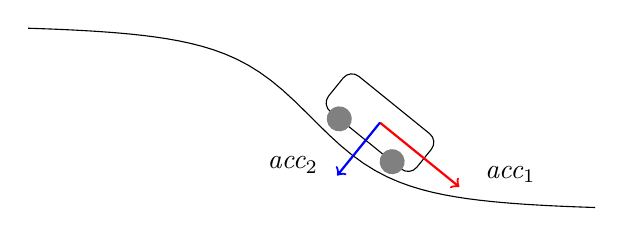
\begin{tikzpicture}[scale=1.2,samples=50,domain=-3:3]
\draw plot (\x,{(-\x/sqrt(\x*\x+1)});
\begin{scope}[xshift=3pt,yshift=4pt,scale=.6,rotate=-39]
\draw[rounded corners] (0,0) -- (0,.8) -- (2, .8) -- (2,0) -- cycle;
\draw[fill,gray] (.4,0) circle[radius=6pt];
\draw[fill,gray] (1.6,0) circle[radius=6pt];
\draw[->,red,thick] (1,.4) -- +(1.8,0);
\draw[->,blue,thick] (1,.4) -- +(0,-1.2);
\end{scope}
\node at (2.1,-.6) {$\textit{acc}_1$};
\node at (-.2,-.5) {$\textit{acc}_2$};
\end{tikzpicture}
\end{center}
\caption{A robot with accelerometers moving in difficult terrain}\label{fig.slopes}
\end{figure}

Figure~\ref{fig.slopemes} shows data acquired during a training session as the robot moves down a slope. When the operator of the training session determines that the robot is stable (class $C_1$), she initiates a measurement indicated by a red $\times$; when she determines that the robot is in a dangerous situation (class $C_2$), she initiates a measurement indicated by a black triangle. The challenge is to find a way of distinguishing samples of the two classes.

\begin{figure}
\begin{center}
\includegraphics[width=\textwidth]{slope-allmu.pdf}
\end{center}
\caption{Detecting a dangerous slope using data from the accelerometers}\label{fig.slopemes}
\end{figure}

The dashed lines in the figure show the means for the two data sets. It is clear that they do not help us classify the data because of the large overlap between the two sets of samples. Furthermore, LDA is not appropriate because there is no similarity in the distributions: samples when the robot is stable appear in many parts of the plot, while samples from dangerous situations are concentrated in a small area around their mean.

\subsection{Classification with perceptrons}

A \emph{perceptron} is an artificial neuron with a specific structure (Fig.~\ref{fig.perceptron}). It has a summation unit with inputs $\{x_1,\ldots,x_n\}$ and each input $x_i$ is multiplied by a factor $w_i$ before summation. An additional input $x_0$ has the constant value $1$ for setting a bias independent of the inputs. The output of the perceptron is obtained by applying a function $f$ to the result of the addition.

\begin{figure}
\begin{center}
\begin{tikzpicture}%
[node distance=1.5cm and 2cm, nn/.style={circle,draw,minimum size=16pt}]
% Inputs
\node at (0,4) (i1) {};
\node at (0,3) (i2) {};
\node at (0,2) (i3) {};
\node at (0,0) (in) {};
\foreach \y in {.5,.75,1,1.25,1.5} \node at (0,\y) {$.$};
\foreach \i in {i1,i2,i3,in}
  \draw (\i) [yshift=-4pt,xshift=-1pt] arc[start angle=-90, end angle=90, radius=4pt] {};
% Neuron
\pic at (4,2) { nnnode={neuron} };
\% Output
\node (output) [node distance=1.5cm and 1cm,right=of neuron] {};
\draw[->] (neuron) -- (output) node {$y$};
% Arrows to neuron
\draw[->] (i1) node [xshift=-12pt] {$x_0=1$} -- node[fill=white] {$w_0$} (neuron);
\draw[->] (i2) node [xshift=-5pt] {$x_1$} -- node[fill=white] {$w_1$} (neuron);
\draw[->] (i3) node [xshift=-5pt] {$x_2$} -- node[fill=white] {$w_2$} (neuron);
\draw[->] (in) node [xshift=-5pt] {$x_n$} -- node[fill=white] {$w_n$} (neuron);
\end{tikzpicture}
\end{center}
\caption{A perceptron}\label{fig.perceptron}
\end{figure}

When used as a classifier, the inputs to the perceptron are the values returned by the sensors for a sample to be classified and the output will be one of two values that indicate the class to which the sample is assigned. Usually, the output function $f$ is just the sign of the weighted sum:
\begin{equation}
y=sign\left(\,\sum_{i=0}^{n} w_i\,x_i\,\right)=\pm 1\,,\label{eq.perceptron-output}
\end{equation}
where one class corresponds to $+1$ and the other to $-1$.

The data are normalized so that all inputs are in the same range, usually $-1\leq x_i\leq +1$. The data in Fig.~\ref{fig.slopemes} can be normalized by dividing each value by $30$.

Given a set of input values $\{x_0=1,x_1,\ldots,x_n\}$ of a sample, the object of a training session is to find a set of weights $\{w_0,w_1,\ldots,w_n\}$ so that the output will be the value $\pm 1$ that assigns the sample to the correct class.

If the sample is close to the border between two classes, the weighted sum will be close to zero. Therefore, a perceptron is also a linear classifier: to distinguish between outputs of $\pm 1$, the discriminant dividing the two classes is defined by the set of weights giving an output of zero:
\[
\sum_{i=0}^{n} w_i\,x_i=0\,,
\]
or
\begin{equation}
w_0 + w_1x_1 + \cdots + w_nx_n = 0\,.\label{eq.perceptron-disc}
\end{equation}
The presentation of LDA for a two-dimensional problem ($n=2$) led to Eq.~\ref{eq.diseq}, which is the same as Eq.~\ref{eq.perceptron-disc} when $c=-w_0$. The difference between the two approaches is in the way the weights are obtained: in LDA statistics are used while for perceptrons they result from an iterative learning process.

\subsection{Learning by a perceptron}

The iterative search for values of the weights $\{w_0,w_1,\ldots,w_n\}$ starts by setting them to a small value such as $0.1$. During the learning phase, a set of samples is presented to the perceptron, together with the expected output (the class) for each element of the set. The set of samples must be constructed randomly and include elements from all the classes; furthermore, the elements from a single class must also be chosen randomly. This is to prevent the learning algorithm from generating a discriminant that is optimal in one specific situation, and to ensure that the process converges rapidly to an overall optimal discriminant, rather than spending too much time optimizing for specific cases.

The adjustment of the weights is computed as follows:
\begin{equation}
w_i(t+1) = w_i(t) + \eta \,x_i \,y\,,\;\;0\leq i \leq n\,.\label{eq.perceptron-learn}
\end{equation}
This is essentially the Hebbian rule for ANNs (Eq.~\ref{eq.hebbian}). $w_i(t)$ and $w_i(t+1)$ are the $i$'th weights before and after the correction, $\eta$ defines the learning rate, $x_i$ is the normalized input, and $y$ is the desired output. Since the sign function is applied to the sum of the weighted inputs, $y$ is $1$ or $-1$, except on the rare occasions where the sum is exactly zero. 

Eq.~\ref{eq.perceptron-learn} corrects the weights by adding or subtracting a value that is proportional to the input, where the coefficient of proportionality is the learning rate. A small value for the learning rate means that the corrections to the weights will be in small increments, while a high learning rate will cause the corrections to the weights to be in larger increments. Once learning is completed, the weights are used to classify subsequent samples.

Algorithms~\ref{alg.perceptron1}--\ref{alg.perceptron2} are a formal description of classification by perceptrons. The constant $N$ is the size of the set of samples for the learning phase, while $n$ is the number of sensor values returned for each sample.

\begin{figure}
\begin{alg}{Classification by a perceptron (learning phase)}{perceptron1}
\hline
&\idv{}float array[$N$,$n$] $\vec{X}$&// Set of samples\\
&\idv{}float array[$n+1$] $\vec{w}$ \ass{} $[0.1,0.1,\ldots]$&// Weights\\
&\idv{}float array[$n$] $\vec{x}$&// Random sample\\
&\idv{}integer $c$&// Class of the random sample\\
&\idv{}integer $y$&// Output of the perceptron\\
\hline
\stl{}&loop until learning terminated&\\ 
\stl{}&\idc{}$\vec{x}$ \ass random element of $\vec{X}$&\\
\stl{}&\idc{}$c$ \ass class to which $\vec{x}$ belongs&\\
\stl{}&\idc{}$y$ \ass output according to Eq.~\ref{eq.perceptron-output}&\\
\stl{}&\idc{}if $y$ does not correspond to class $c$&\\
\stl{}&\idc{}\idc{}adjust $w_i$ according to Eq.~\ref{eq.perceptron-learn}&\\
\stl{}&Output $\vec{w}$&\\
\end{alg}
\end{figure}

\begin{figure}
\begin{alg}{Classification by a perceptron (recognition phase)}{perceptron2}
&\idv{}float $\vec{w}$ \ass weights from the learning phase&\\
&\idv{}float $\vec{x}$&\\
&\idv{}integer $y$&\\
\hline
\stl{}&loop&\\
\stl{}&\idc{}$\vec{x}$ \ass new sample&\\
\stl{}&\idc{}$y$ \ass output of perceptron for $\vec{x},\vec{w}$&\\
\stl{}&\idc{}if $y=1$&\\
\stl{}&\idc{}\idc{}assign $\vec{x}$ to class $C_1$&\\
\stl{}&\idc{}else if $y=-1$&\\
\stl{}&\idc{}\idc{}assign $\vec{x}$ to class $C_2$&\\
\end{alg}
\end{figure}

When should the learning phase be terminated? One could specify an arbitrary value, for example: terminate the learning phase when $98\%$ of the samples are classified correctly. However, it may not be possible to achieve this level. A better method is to terminate the learning phase when the magnitudes of the corrections to the weights become small.

\subsection{Numerical example}

We return to the robot that is learning to avoid dangerous slopes and apply the learning algorithm to the data in Fig.~\ref{fig.slopemes}. The perceptron has three inputs: $x_0$ which always set to $1$, $x_1$ for the data from the front/back accelerometer, and $x_2$ for the data from the up/down accelerometer. The data is normalized by dividing each sample by $30$ so that values will be between $0$ and $1$. We specify that an output of $1$ corresponds to class $C_1$ (stable) and an output of $-1$ corresponds to class $C_2$ (dangerous).

Select a random sample from the input data, for example, a sample in class $C_1$ whose sensor values are $x_{1}=14$ and $x_{2}=18$. The normalized input is $x_{1}=14/30=0.47$ and $x_{2}=18/30=0.6$. The output of the perceptron with initial weights $0.1$ is:
\begin{eqnarray*}
y &=& \mathit{sign}(w_0\times 1 + w_1x_1 + w_2x_2)\\
&=& \mathit{sign}(0.1\times 1 + 0.1\times 0.47 + 0.1\times 0.6)\\
&=& \mathit{sign}(0.207)\\
&=& 1\,.
\end{eqnarray*}
This output is correct so the weights need not be corrected. Now choose a random sample in class $C_2$ whose sensor values are  $x_{1}=17$ and $x_{2}=15$. The normalized input is $x_{1}=17/30=0.57$ and $x_{2}=15/30=0.5$. The output of the perceptron is:
\begin{eqnarray*}
y &=& \mathit{sign}(w_0\times 1 + w_1x_1 + w_2x_2)\\
&=& \mathit{sign}(0.1\times 1 + 0.1\times 0.57 + 0.1\times 0.5)\\
&=& \mathit{sign}(0.207)\\
&=& 1\,.
\end{eqnarray*}
This output is not correct: the sample is from class $C_2$ which corresponds to $-1$. The weights are now adjusted using Eq.~\ref{eq.perceptron-learn} with a learning rate $\eta = 0.1$:
\[
\spacearray
\begin{array}{lclclcl}
w_0(t+1) &=& w_0(t) + \eta \,x_0 y &=& 0.1 + 0.1\times 1\times -1 &=& 0 \\
w_1(t+1) &=& w_1(t) + \eta \,x_1 y &=& 0.1 + 0.1\times 0.57\times-1 &=& 0.043 \\
w_2(t+1) &=& w_2(t) + \eta \,x_2 y &=& 0.1 + 0.1\times 0.5\times -1 &=& 0.05\,.
\end{array}
\]
These will be the new weights for the next iteration. If we continue for $2000$ iterations, the weights evolve as shown in Fig.~\ref{fig.weights-fixeta}. At the end of the learning process, the weights are:
\[
w_0 = -0.1,\;\;\; w_1 = -0.39,\;\;\; w_2 = 0.53\,.
\]

\begin{figure}[bt]
\begin{center}
\includegraphics[width=0.8\textwidth]{weights.pdf}
\end{center}
\caption{Evolution of the weights for learning by a perceptron}\label{fig.weights-fixeta}
\end{figure}

These weights can now be used by the recognition phase of the classification Algorithm~\ref{alg.perceptron2}. The discriminant line built by the perceptron (Eq.~\ref{eq.perceptron-disc}) is:
\[
-0.1 -0.39x_1 + 0.53x_2 = 0\,.
\]
The coordinates of this line are the normalized values, but they can be transformed back into the raw values obtained from the accelerometers. The line is shown in Fig.~\ref{fig.perceptron-dis} and considering the large overlap of the classes, it does a reasonably good job of distinguishing between them.

\begin{figure}
\begin{center}
\includegraphics[width=0.9\textwidth]{perceptron-discrim.pdf}
\end{center}
\caption{Discriminant line computed from the perceptron weights}\label{fig.perceptron-dis}
\end{figure}

\subsection{Tuning the parameters of the perceptron}

The performance of a perceptron is determined by the number of iterations and the learning rate. Figure~\ref{fig.weights-fixeta} shows that there is a strong variation in the weights at the beginning, but the weights stabilize as the number of iterations increases. Thus it is relatively simple to monitor the weights and terminate the computation when the weights stabilize.

This evolution of the weights depends strongly on the learning rate. Increasing the learning rate speeds the variation at the beginning, but strong corrections are not beneficial when the weights begin to stabilize. From Fig.~\ref{fig.weights-fixeta}, it is clear that even at the end of the run, there are significant variations in the weights which oscillate around the optimal value. This suggests that we reduce the learning rate to reduce the oscillations, but doing so will slow down the convergence to the optimal weights at the beginning of the learning phase.

The solution is to use a variable learning rate that is not constant. It should start out large to encourage rapid convergence to the optimal values, and then become smaller to reduce oscillations. For example, we can start with the learning rate of $0.1$ and then decrease it continually using the equation:
\[
\eta\,(t+1) = \eta\,(t) \times 0.997\,.
\]
Figure~\ref{fig.perceptron-dis-etavar} shows the evolution of the weights when this variable learning rate is used. The exponential decrease of $\eta$ is also plotted in the figure. A comparison of Fig.~\ref{fig.weights-fixeta} and Fig.~\ref{fig.perceptron-dis-etavar} clearly shows the superiority of the variable learning rate and this improvement is obtained with very little additional computation.
\begin{figure}
\begin{center}
\includegraphics[width=0.9\textwidth]{weights-etavar.pdf}
\end{center}
\caption{Evolution of the weights for learning by a perceptron with a variable learning rate}\label{fig.perceptron-dis-etavar}
\end{figure}

\begin{framed}
\act{Learning by a perceptron}{perceptronlearn}
\begin{itemize}
\item Take a set of measurements of the accelerometers on your robot on various slopes and plot the data. For each sample you will have to decide if the robot is in danger of falling off the slope.
\item Classify the data using a perceptron. What discriminant line do you find?
\item Use a perceptron to classify the gray areas using the data of Activity~\ref{act.LDAchameleon}. What discriminant do you find? Compare the discriminant found by the perceptron to the discriminant found by LDA.
\end{itemize}
\end{framed}

\section{Summary}

Samples of two classes can be distinguished using their means alone or using both the means and the variances. Linear discriminant analysis is a method for classification that is based on computing the covariances between the samples of the classes. LDA performs well only when the distributions of the samples of the classes are similar. When this assumption does not hold, perceptrons can be used. For optimum performance, the learning rate of a perceptron must be adjusted, if possible dynamically during the learning phase.

\section{Further reading}

A detailed mathematical presentation of linear discriminant analysis can be found in Izenman~\cite[Chapter~8]{izenman2008}. Textbooks on machine learning techniques are \cite{harrington2012machine, kubat2015machinelearning}.
